\documentclass[a4j]{jarticle}

\usepackage{amssymb}
\usepackage[dvipdfmx]{graphicx}
\usepackage{subfigure}
\usepackage{here}

\begin{document}

\begin{table}[t]
\begin{center}
{\large LTE 環境における応答遅延特性の時系列モデリングによる分析}\\
Analysis of delay characteristics of connection through LTE by time series analysis\\
令和 2 年 3 月 4 日\\
山本 航平
\end{center}
\end{table}

\section{進捗報告}
\begin{itemize}
\item 5 月開催 IN 研究会への参加申し込みを行いました.
\item \lq{}\lq{}aws.amazon.com\rq{}\rq{},\lq{}\lq{}news.yahoo.co.jp\rq{}\rq{},\lq{}\lq{}13.114.202.235(AWS サーバ)\rq{}\rq{}を対象に計測実験を行いました.
\item traceroute 結果より通信経路を調べました.
\item fBm(fractional Brownian motion : 非整数ブラウン運動)モデルへの適用を検討しています.
\end{itemize}

\section{アブストラクト}
産業用モニタリングシステムにおける運用管理コストの低減のため,迅速な障害検知・予測,ならびに原因の特定と対処法の提示が求められている.
その実現にむけて,無線機器からサーバまでのLTE回線を含む通信路について,異なる場所や時間帯において応答遅延の計測を行った.
本稿では,遅延の変動特性や,場所や曜日,時間帯に依存した傾向の有無について,時系列モデルを用いたクラスタリングによって分析した結果を示す.

\textbf{キーワード : }LTE(Long Term Evolution),応答遅延,障害検知,時系列モデリング\\
\section{計測実験の設定}
本報告では図 \ref{exp} に示す構成で計測実験を行った.
モニタリングシステムにおける無線端末としては LTE モジュールとして Quectel 社製 EC21-J を搭載した Raspberry Pi を用いた.
また,LTE 回線としては IIJ モバイル社のサービスタイプ D 定額プランライト(いちねん プリペイド)を用いた.
IIJ モバイル社は他の通信事業者から通信回線を借り受け,サービスを提供している MVNO(Mobile Virtual Network Operator)であり,サービスタイプ D では NTT ドコモ社の回線を使用している.
月あたり通信量が 3GB を超過すると通信速度が 256kbps に制限されるが,本実験中には速度制限は課されなかった.

クラウドサーバとしては AWS サーバ(13.114.202.235)や AWS のウェブサーバ(aws.amazon.com),yahoo ニュースのサーバ(news.yahoo.co.jp)を用い,Raspberry Pi から traceroute や ping を用いて経路や応答遅延を計測した.
自動的に計測データを取得できるよう,Raspberry Pi 上で動作する Raspbian において計測用のスクリプトを用いることで,5 秒または 15 秒毎に時刻を取得し,続けて ping (パケットサイズ 60 バイト, ICMP ECHO メッセージ,パケット数 1 )を実行し,続けて traceroute (パケットサイズ 60 バイト, TCP パケット,パケット数 1 )を実行した.
計測時刻,tracerouteの出力,pingの出力をログデータとして取り出し,分析を行った.
また,日時が応答遅延に与える影響を調べるため,様々な時間帯で計測を行った.
計測日時,計測内容を表 \ref{keisoku} に示す.
計測場所は若宮研究室内,測定周期は 15 秒,計測内容はすべて ping と traceroute とした.
\begin{figure}[tb]
\centering
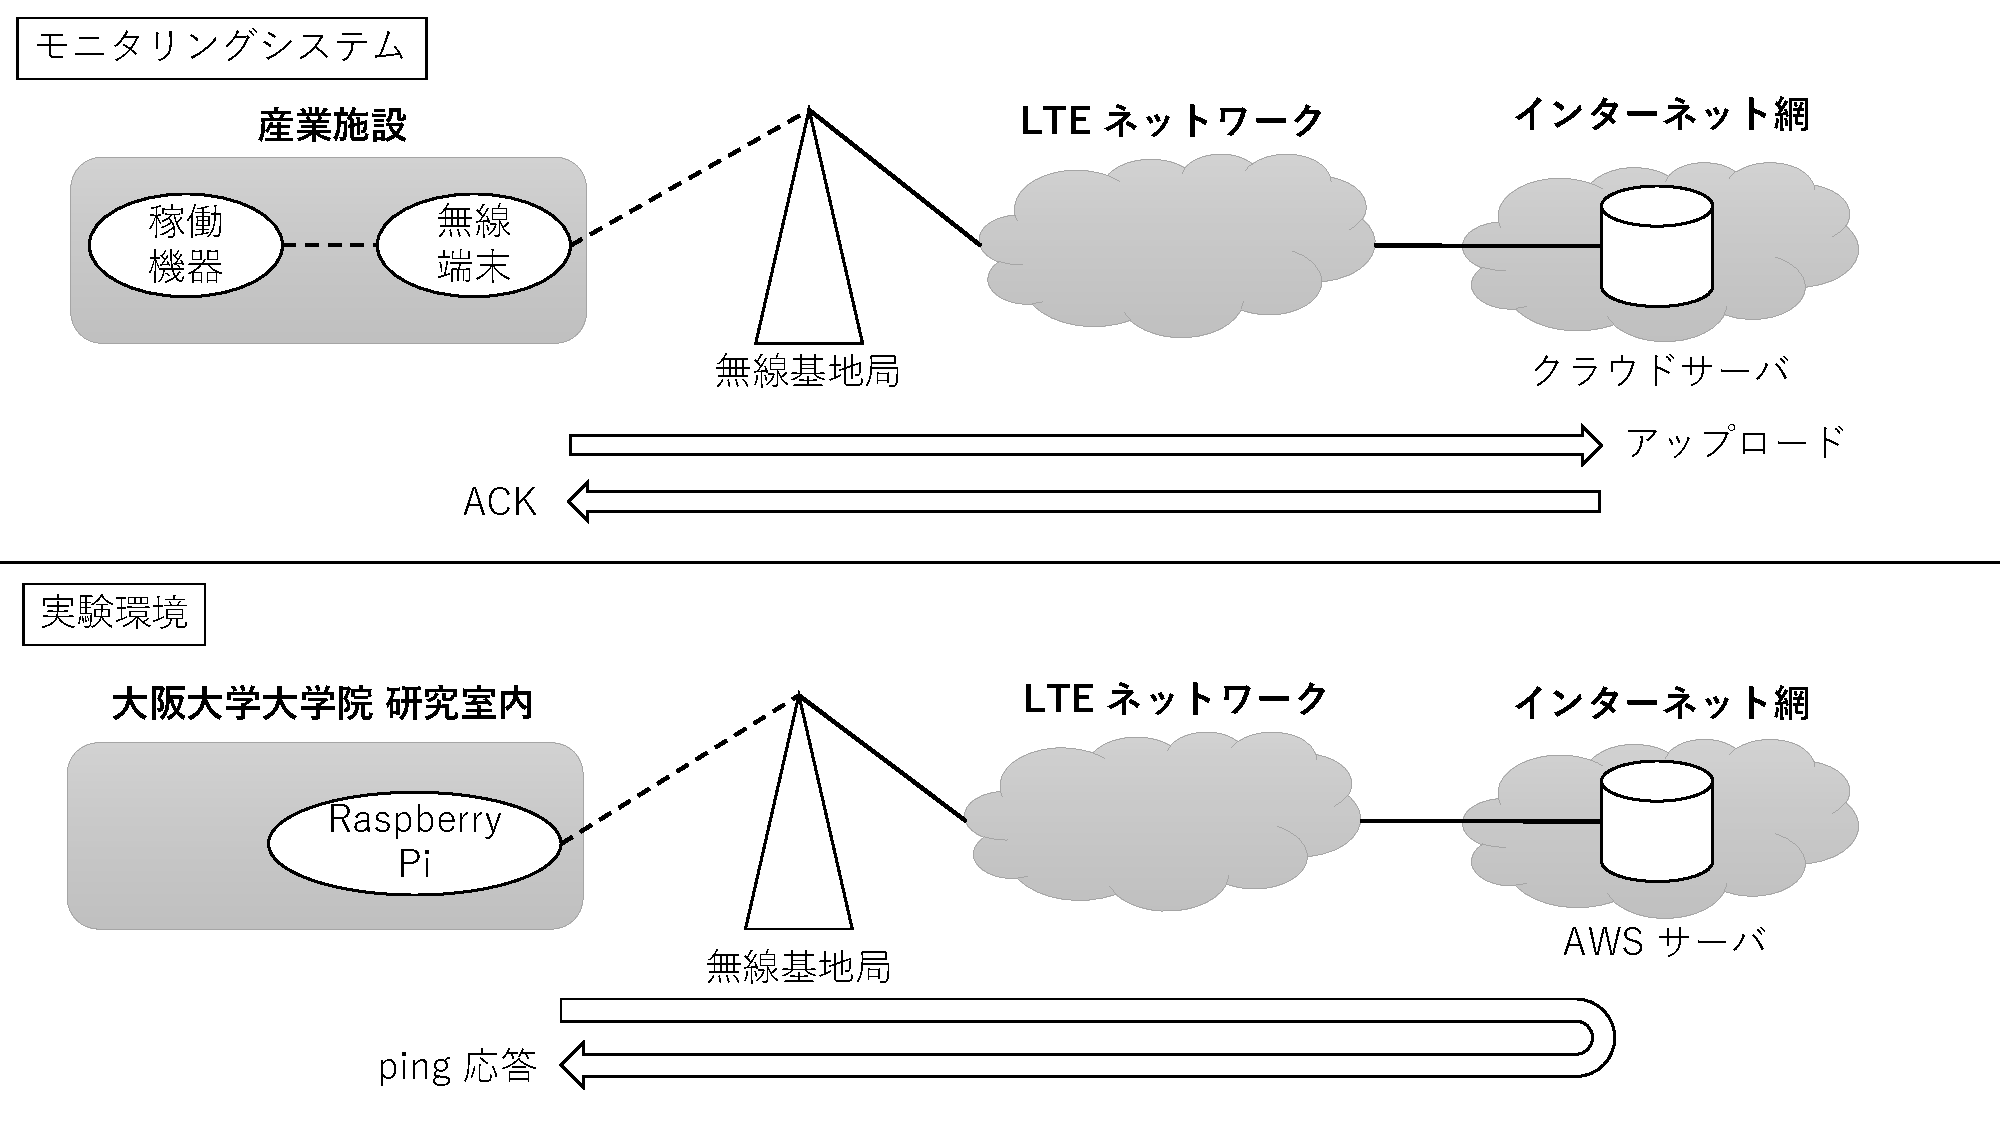
\includegraphics[width=10.0cm]{../figure/experiment.pdf}
\caption{モニタリングシステムと実験設定の対応}
\label{exp}
\end{figure}

\begin{table}[tb]
\centering
\caption{実験の計測日時,対象}
\label{keisoku}
\begin{tabular}{|p{7cm}|p{7cm}|}
\hline
計測日時&対象\\
\hline
2/22(土)から 2/28(金)までのそれぞれ 3:00-4:00,7:00-8:00,12:00-13:00,17:00-18:00,20:00-21:00& AWS のウェブサーバ(aws.amazon.com)\\
\hline
2/22(土)から 3/3(火)までのそれぞれ 3:00-4:00,7:00-8:00,12:00-13:00,17:00-18:00,20:00-21:00& yahoo ニュースのサーバ(news.yahoo.co.jp)\\
\hline
2/29(土)から 3/3(火)までのそれぞれ 3:00-4:00,7:00-8:00,12:00-13:00,17:00-18:00,20:00-21:00&  AWS サーバ(13.114.202.235)\\
\hline
\end{tabular}
\end{table}

\section{計測結果}
2/22(土)から 3/3(火)までの計測結果を図 \ref{data-start} から図 \ref{data-end} に示す.
ping 応答遅延の計測データを縦軸に取り,横軸に計測開始時のものから 1 から順に割り振ったインデックス $t$ を取った.
縦軸の範囲は 0ms から 400ms までとし,100ms から 400ms までの区間は縮小してある.
また,各図の上にそのデータの平均と分散を記した.

\begin{figure}[tb]
\begin{center}
\subfigure[3:00 - 4:00]{
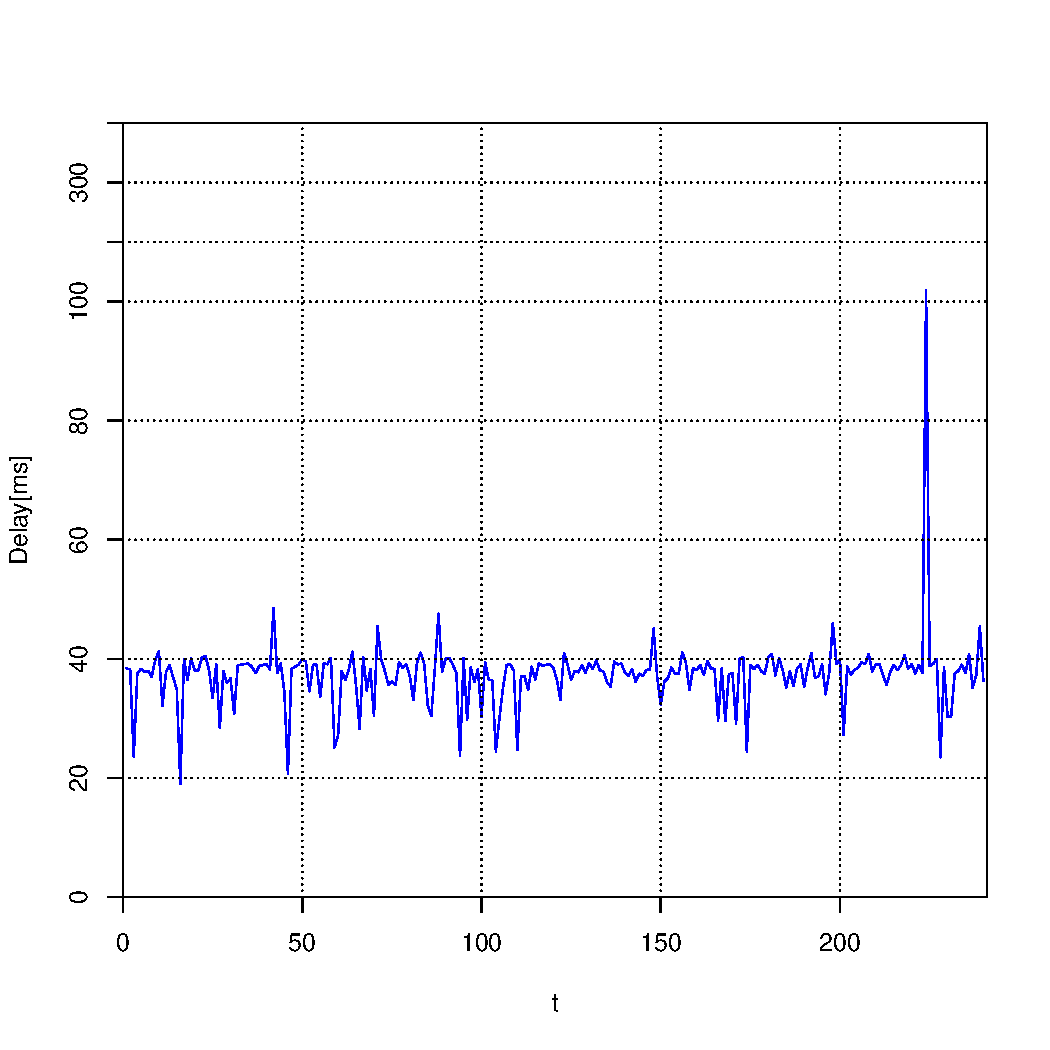
\includegraphics[width=.3\columnwidth]{C:/master/mstudy/analysis/plot/aws.amazon.com/20200222_030001-plot.pdf}
}~
\subfigure[7:00 - 8:00]{
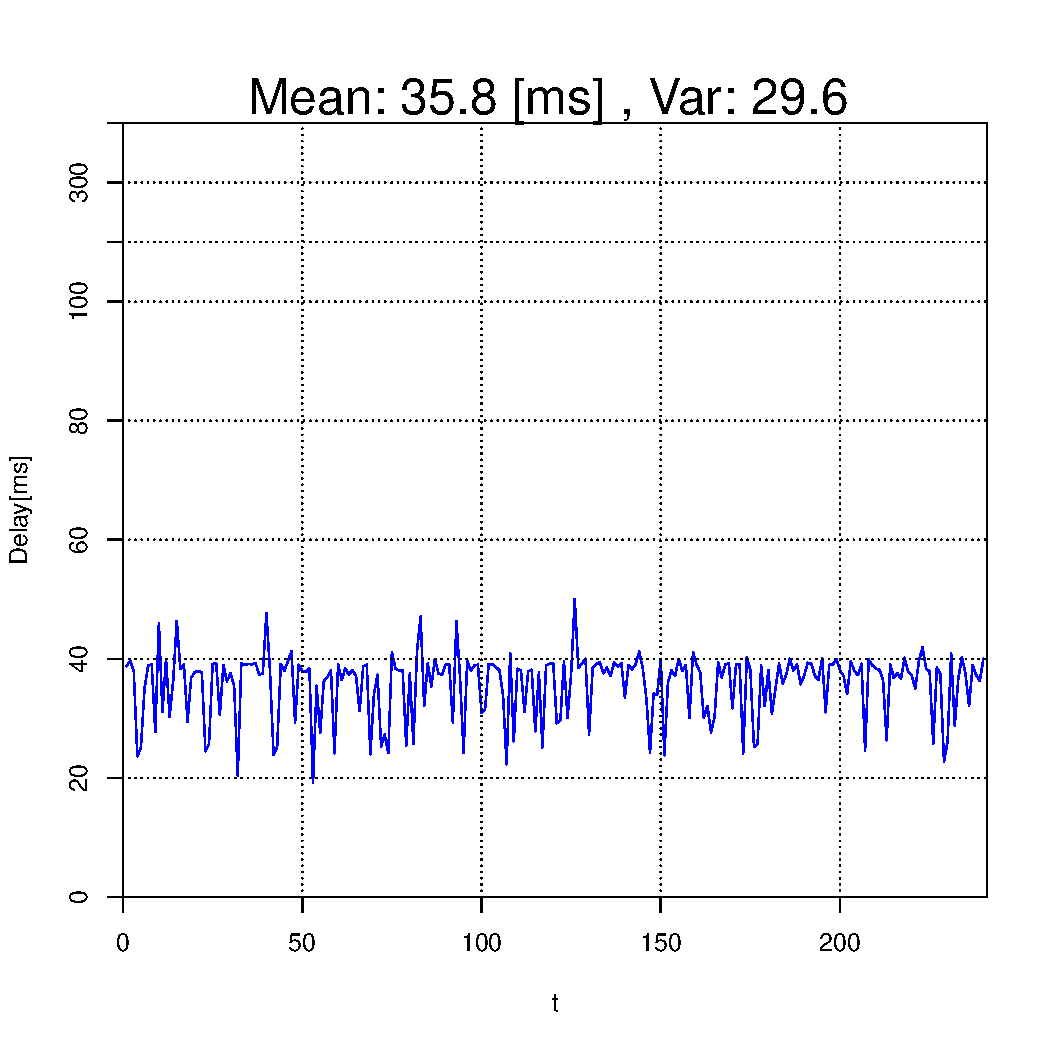
\includegraphics[width=.3\columnwidth]{C:/master/mstudy/analysis/plot/aws.amazon.com/20200222_070002-plot.pdf}
}~
\subfigure[12:00 - 13:00]{
\includegraphics[width=.3\columnwidth]{C:/master/mstudy/analysis/plot/aws.amazon.com/20200222_120001-plot.pdf}
}\\
\subfigure[17:00 - 18:00]{
\includegraphics[width=.3\columnwidth]{C:/master/mstudy/analysis/plot/aws.amazon.com/20200222_170002-plot.pdf}
}~
\subfigure[20:00 - 21:00]{
\includegraphics[width=.3\columnwidth]{C:/master/mstudy/analysis/plot/aws.amazon.com/20200222_200001-plot.pdf}
}
\caption{2月22日(土) aws.amazon.com を対象}
\label{data-start}

\subfigure[3:00 - 4:00]{
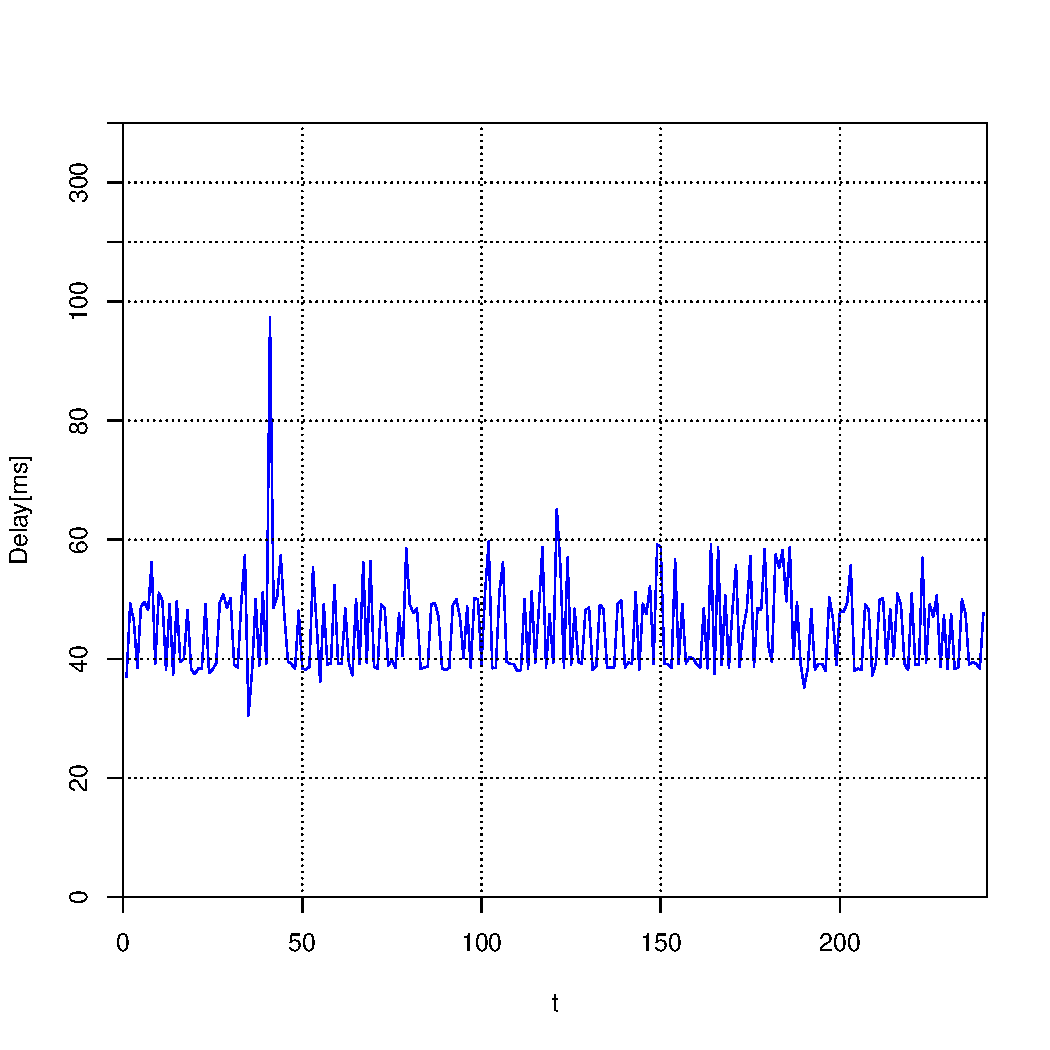
\includegraphics[width=.3\columnwidth]{C:/master/mstudy/analysis/plot/news.yahoo.co.jp/20200222_030002-plot.pdf}
}~
\subfigure[7:00 - 8:00]{
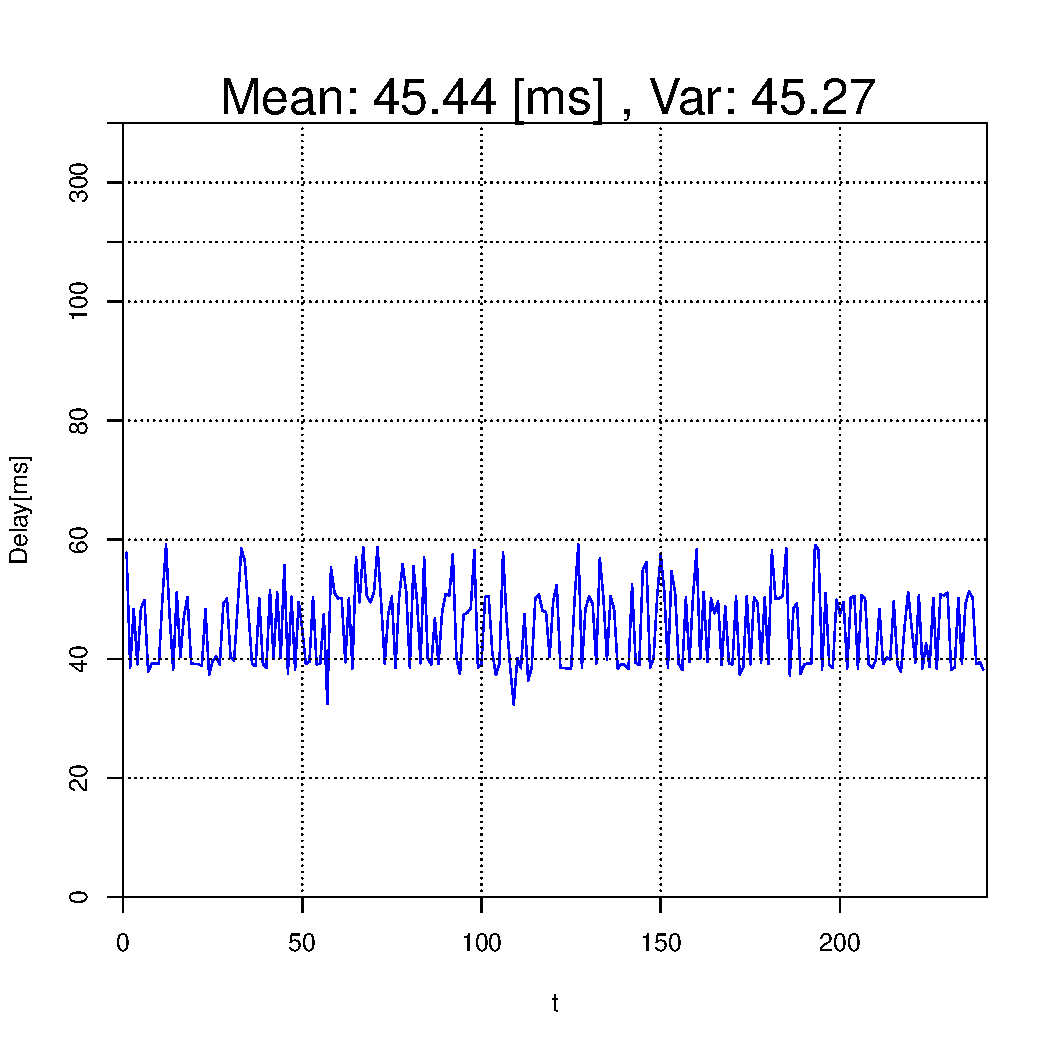
\includegraphics[width=.3\columnwidth]{C:/master/mstudy/analysis/plot/news.yahoo.co.jp/20200222_070001-plot.pdf}
}~
\subfigure[12:00 - 13:00]{
\includegraphics[width=.3\columnwidth]{C:/master/mstudy/analysis/plot/news.yahoo.co.jp/20200222_120001-plot.pdf}
}\\
\subfigure[17:00 - 18:00]{
\includegraphics[width=.3\columnwidth]{C:/master/mstudy/analysis/plot/news.yahoo.co.jp/20200222_170002-plot.pdf}
}~
\subfigure[20:00 - 21:00]{
\includegraphics[width=.3\columnwidth]{C:/master/mstudy/analysis/plot/news.yahoo.co.jp/20200222_200001-plot.pdf}
}
\caption{2月22日(土) news.yahoo.co.jp を対象}
\end{center}
\end{figure}

\begin{figure}[tb]
\begin{center}
\subfigure[3:00 - 4:00]{
\includegraphics[width=.3\columnwidth]{C:/master/mstudy/analysis/plot/aws.amazon.com/20200223_030001-plot.pdf}
}~
\subfigure[7:00 - 8:00]{
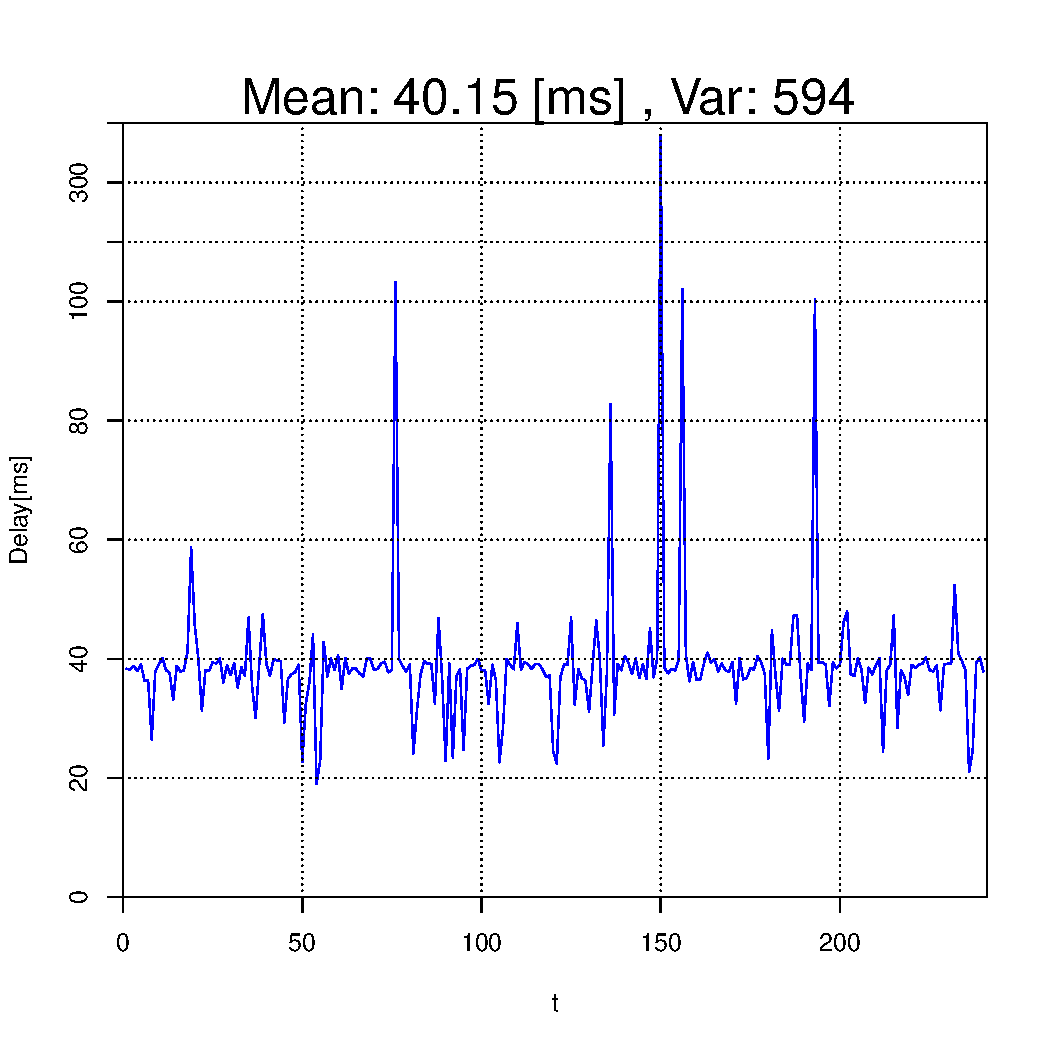
\includegraphics[width=.3\columnwidth]{C:/master/mstudy/analysis/plot/aws.amazon.com/20200223_070001-plot.pdf}
}~
\subfigure[12:00 - 13:00]{
\includegraphics[width=.3\columnwidth]{C:/master/mstudy/analysis/plot/aws.amazon.com/20200223_120001-plot.pdf}
}\\
\subfigure[17:00 - 18:00]{
\includegraphics[width=.3\columnwidth]{C:/master/mstudy/analysis/plot/aws.amazon.com/20200223_170001-plot.pdf}
}~
\subfigure[20:00 - 21:00]{
\includegraphics[width=.3\columnwidth]{C:/master/mstudy/analysis/plot/aws.amazon.com/20200223_200001-plot.pdf}
}
\caption{2月23日(日) aws.amazon.com を対象}

\subfigure[3:00 - 4:00]{
\includegraphics[width=.3\columnwidth]{C:/master/mstudy/analysis/plot/news.yahoo.co.jp/20200223_030001-plot.pdf}
}~
\subfigure[7:00 - 8:00]{
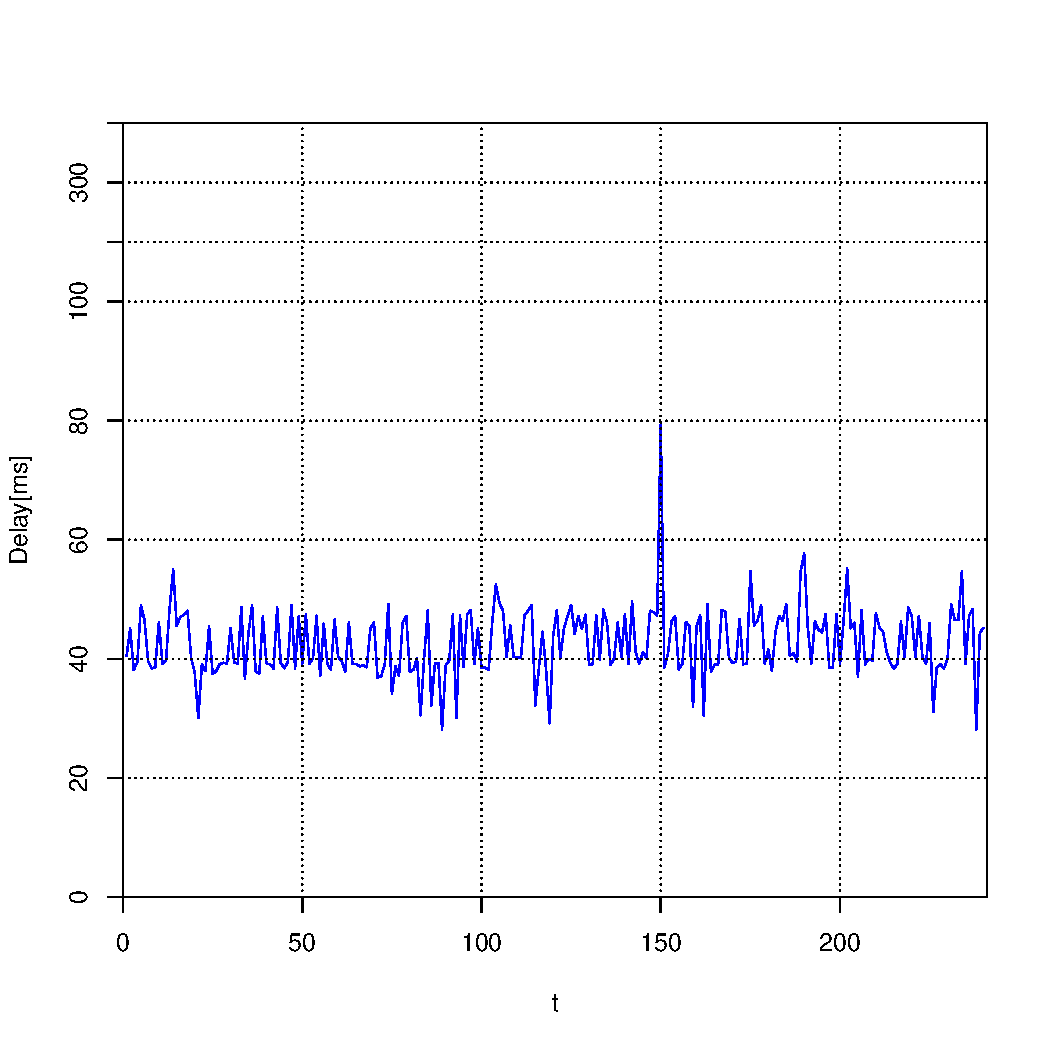
\includegraphics[width=.3\columnwidth]{C:/master/mstudy/analysis/plot/news.yahoo.co.jp/20200223_070002-plot.pdf}
}~
\subfigure[12:00 - 13:00]{
\includegraphics[width=.3\columnwidth]{C:/master/mstudy/analysis/plot/news.yahoo.co.jp/20200223_120001-plot.pdf}
}\\
\subfigure[17:00 - 18:00]{
\includegraphics[width=.3\columnwidth]{C:/master/mstudy/analysis/plot/news.yahoo.co.jp/20200223_170001-plot.pdf}
}~
\subfigure[20:00 - 21:00]{
\includegraphics[width=.3\columnwidth]{C:/master/mstudy/analysis/plot/news.yahoo.co.jp/20200223_200001-plot.pdf}
}
\caption{2月23日(日) news.yahoo.co.jp を対象}
\end{center}
\end{figure}

\begin{figure}[tb]
\begin{center}
\subfigure[3:00 - 4:00]{
\includegraphics[width=.3\columnwidth]{C:/master/mstudy/analysis/plot/aws.amazon.com/20200224_030001-plot.pdf}
}~
\subfigure[7:00 - 8:00]{
\includegraphics[width=.3\columnwidth]{C:/master/mstudy/analysis/plot/aws.amazon.com/20200224_070001-plot.pdf}
}~
\subfigure[12:00 - 13:00]{
\includegraphics[width=.3\columnwidth]{C:/master/mstudy/analysis/plot/aws.amazon.com/20200224_120001-plot.pdf}
}\\
\subfigure[17:00 - 18:00]{
\includegraphics[width=.3\columnwidth]{C:/master/mstudy/analysis/plot/aws.amazon.com/20200224_170001-plot.pdf}
\label{aws}
}~
\subfigure[20:00 - 21:00]{
\includegraphics[width=.3\columnwidth]{C:/master/mstudy/analysis/plot/aws.amazon.com/20200224_200001-plot.pdf}
}
\caption{2月24日(月) aws.amazon.com を対象}

\subfigure[3:00 - 4:00]{
\includegraphics[width=.3\columnwidth]{C:/master/mstudy/analysis/plot/news.yahoo.co.jp/20200224_030001-plot.pdf}
}~
\subfigure[7:00 - 8:00]{
\includegraphics[width=.3\columnwidth]{C:/master/mstudy/analysis/plot/news.yahoo.co.jp/20200224_070001-plot.pdf}
}~
\subfigure[12:00 - 13:00]{
\includegraphics[width=.3\columnwidth]{C:/master/mstudy/analysis/plot/news.yahoo.co.jp/20200224_120001-plot.pdf}
}\\
\subfigure[17:00 - 18:00]{
\includegraphics[width=.3\columnwidth]{C:/master/mstudy/analysis/plot/news.yahoo.co.jp/20200224_170001-plot.pdf}
}~
\subfigure[20:00 - 21:00]{
\includegraphics[width=.3\columnwidth]{C:/master/mstudy/analysis/plot/news.yahoo.co.jp/20200224_200001-plot.pdf}
}
\caption{2月24日(月) news.yahoo.co.jp を対象}
\end{center}
\end{figure}


\begin{figure}[tb]
\begin{center}
\subfigure[3:00 - 4:00]{
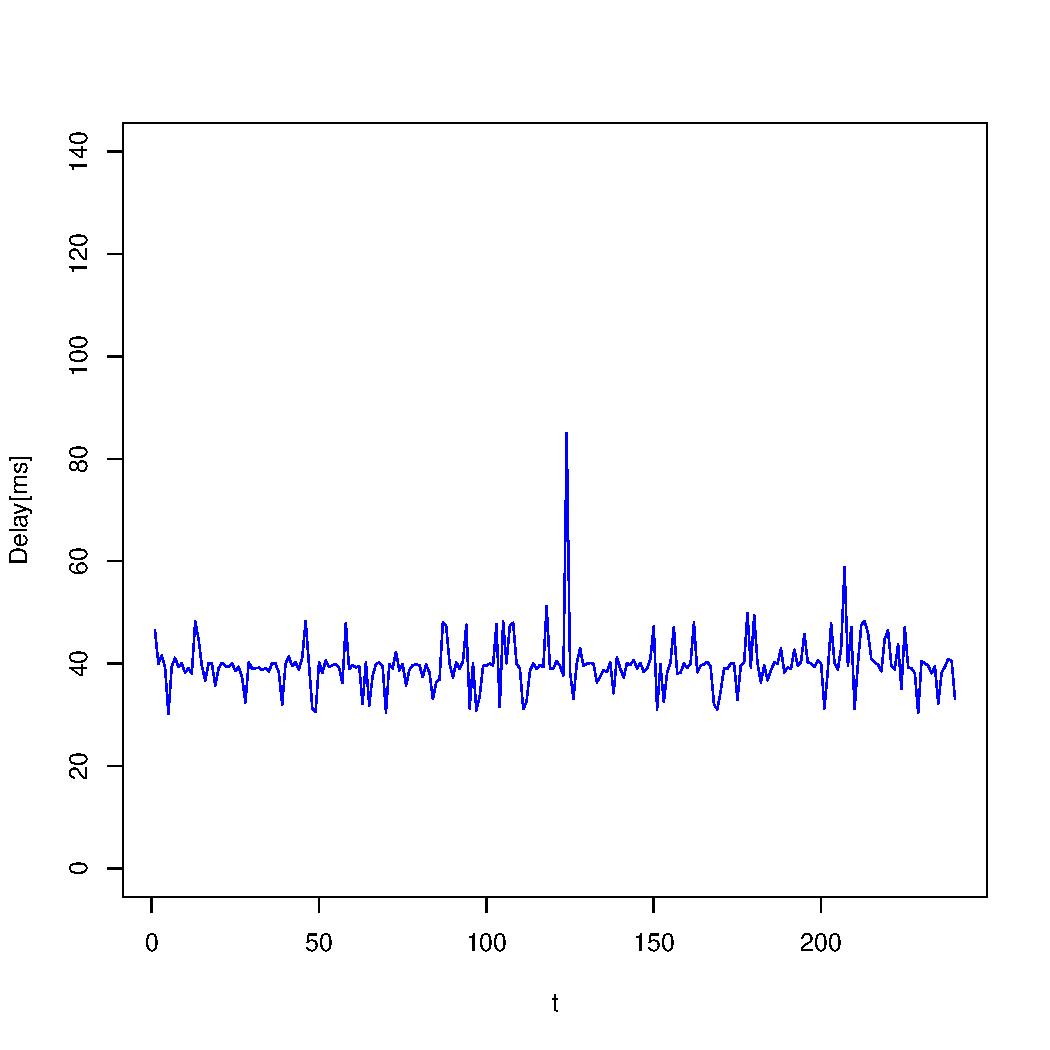
\includegraphics[width=.3\columnwidth]{C:/master/mstudy/analysis/plot/aws.amazon.com/20200225_030001-plot.pdf}
}~
\subfigure[7:00 - 8:00]{
\includegraphics[width=.3\columnwidth]{C:/master/mstudy/analysis/plot/aws.amazon.com/20200225_070001-plot.pdf}
}~
\subfigure[12:00 - 13:00]{
\includegraphics[width=.3\columnwidth]{C:/master/mstudy/analysis/plot/aws.amazon.com/20200225_120001-plot.pdf}
}\\
\subfigure[17:00 - 18:00]{
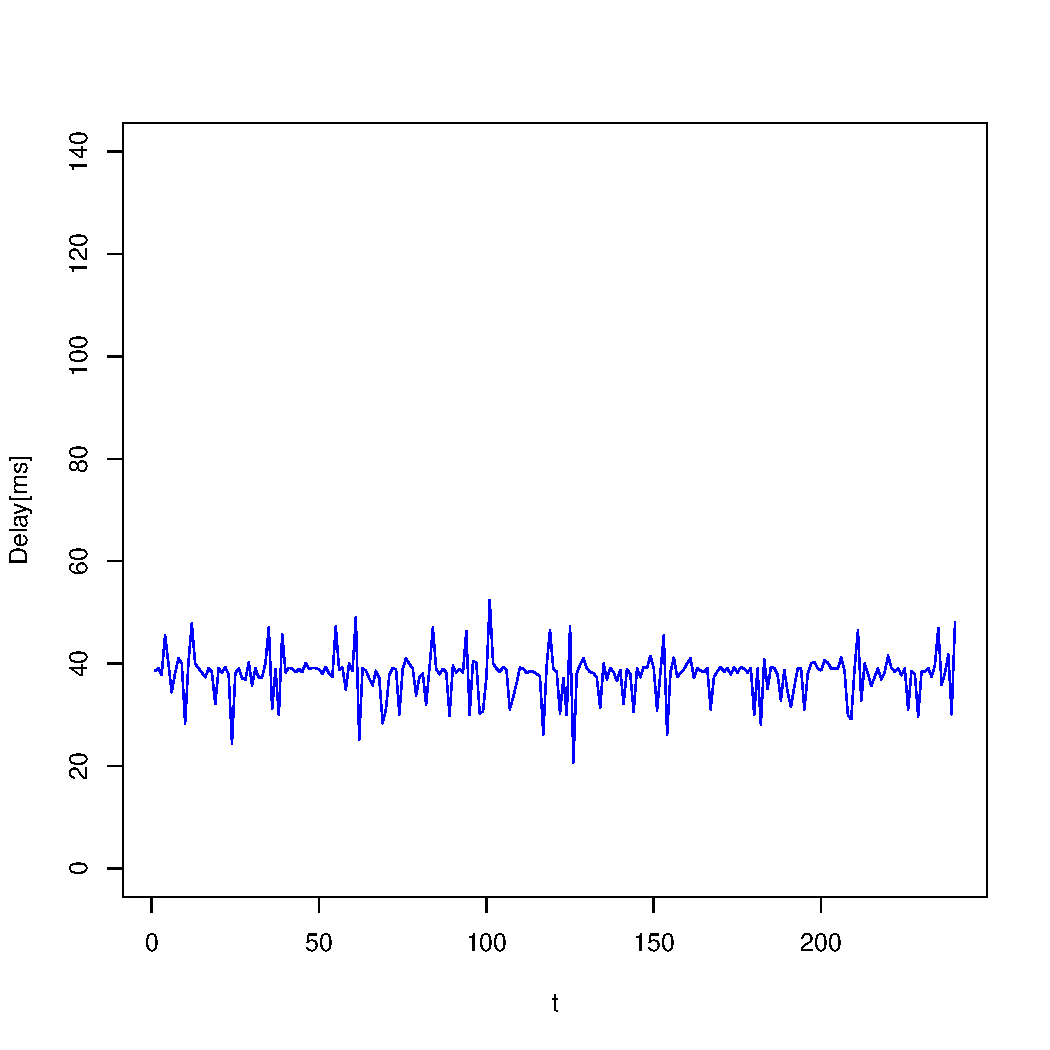
\includegraphics[width=.3\columnwidth]{C:/master/mstudy/analysis/plot/aws.amazon.com/20200225_170002-plot.pdf}
}~
\subfigure[20:00 - 21:00]{
\includegraphics[width=.3\columnwidth]{C:/master/mstudy/analysis/plot/aws.amazon.com/20200225_200001-plot.pdf}
}
\caption{2月25日(火) aws.amazon.com を対象}

\subfigure[3:00 - 4:00]{
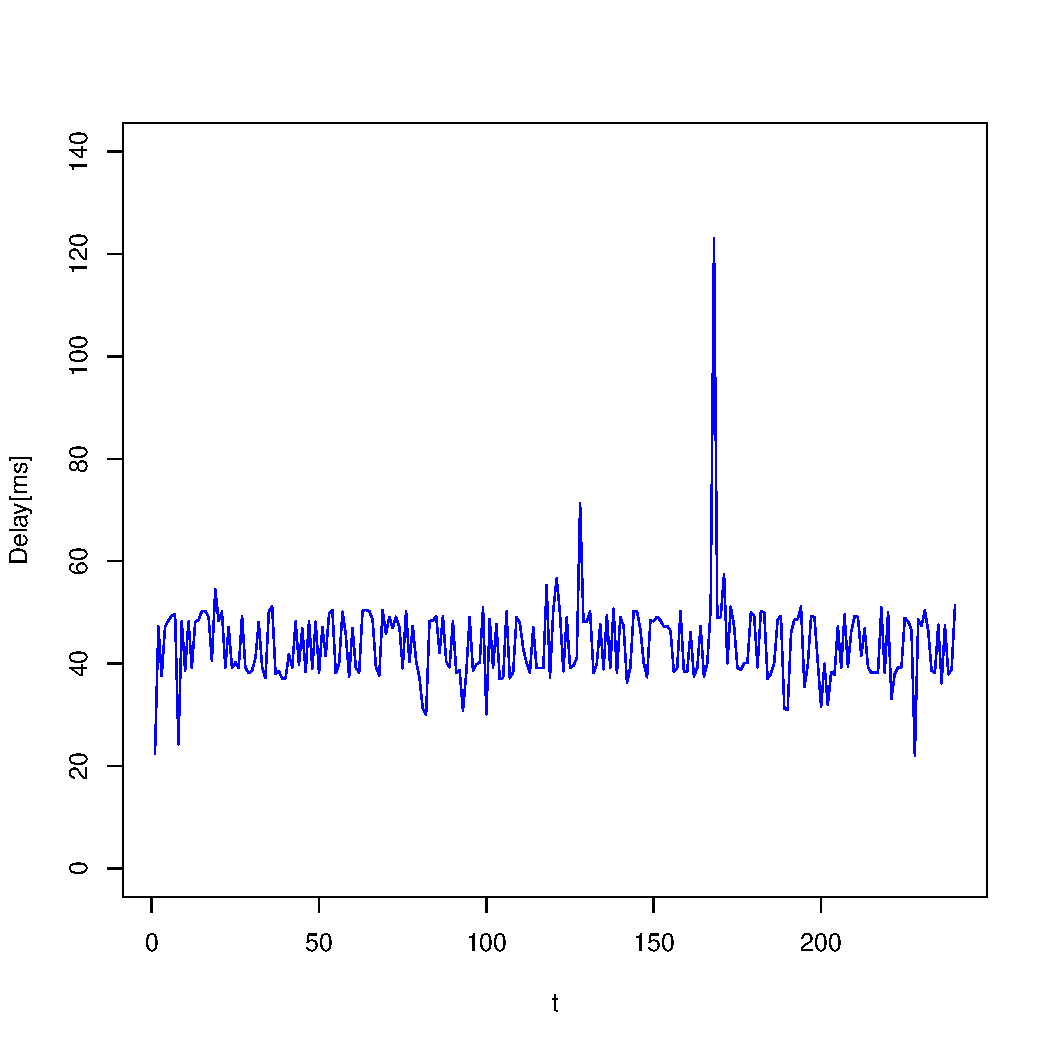
\includegraphics[width=.3\columnwidth]{C:/master/mstudy/analysis/plot/news.yahoo.co.jp/20200225_030002-plot.pdf}
}~
\subfigure[7:00 - 8:00]{
\includegraphics[width=.3\columnwidth]{C:/master/mstudy/analysis/plot/news.yahoo.co.jp/20200225_070001-plot.pdf}
}~
\subfigure[12:00 - 13:00]{
\includegraphics[width=.3\columnwidth]{C:/master/mstudy/analysis/plot/news.yahoo.co.jp/20200225_120001-plot.pdf}
}\\
\subfigure[17:00 - 18:00]{
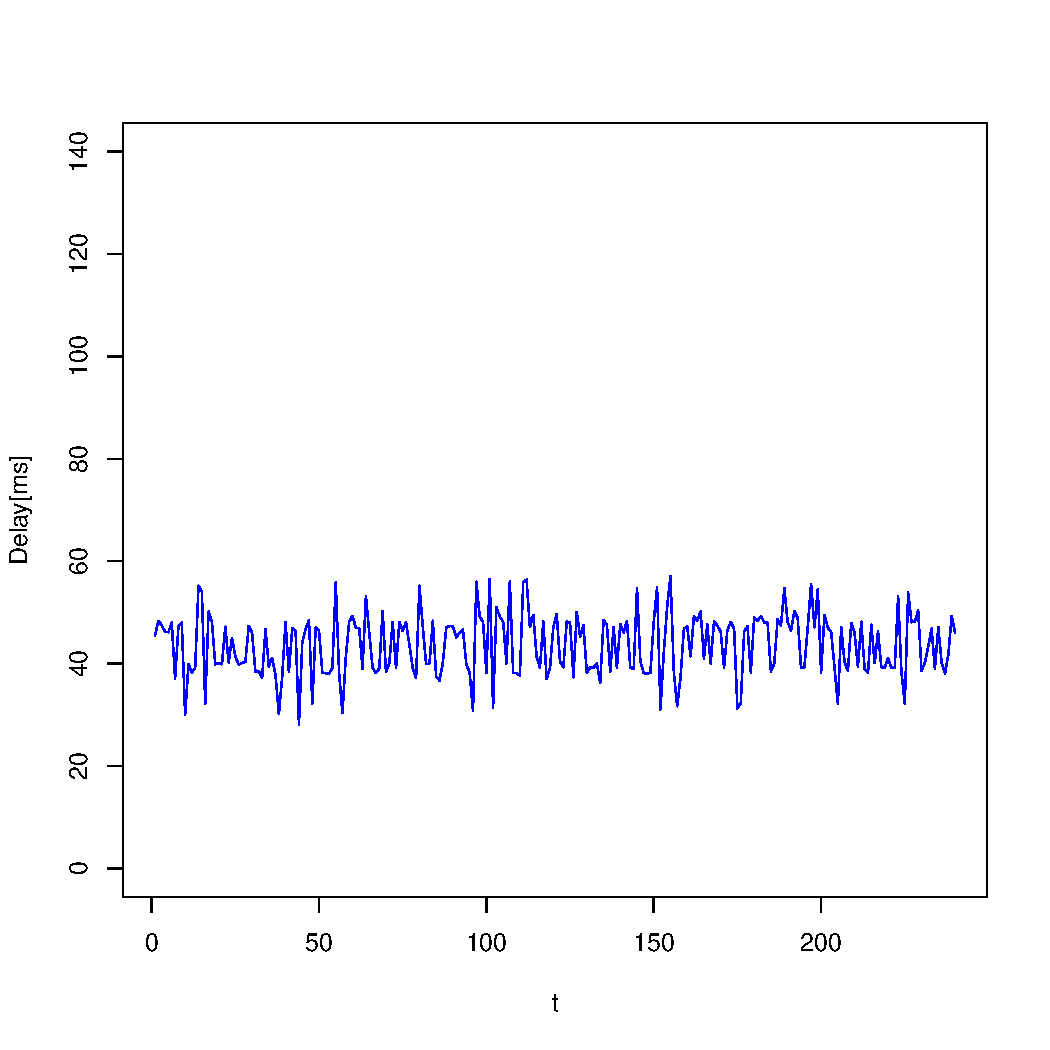
\includegraphics[width=.3\columnwidth]{C:/master/mstudy/analysis/plot/news.yahoo.co.jp/20200225_170001-plot.pdf}
}~
\subfigure[20:00 - 21:00]{
\includegraphics[width=.3\columnwidth]{C:/master/mstudy/analysis/plot/news.yahoo.co.jp/20200225_200001-plot.pdf}
}
\caption{2月25日(火) news.yahoo.co.jp を対象}
\end{center}
\end{figure}

\begin{figure}[tb]
\begin{center}
\subfigure[3:00 - 4:00]{
\includegraphics[width=.3\columnwidth]{C:/master/mstudy/analysis/plot/aws.amazon.com/20200226_030001-plot.pdf}
}~
\subfigure[7:00 - 8:00]{
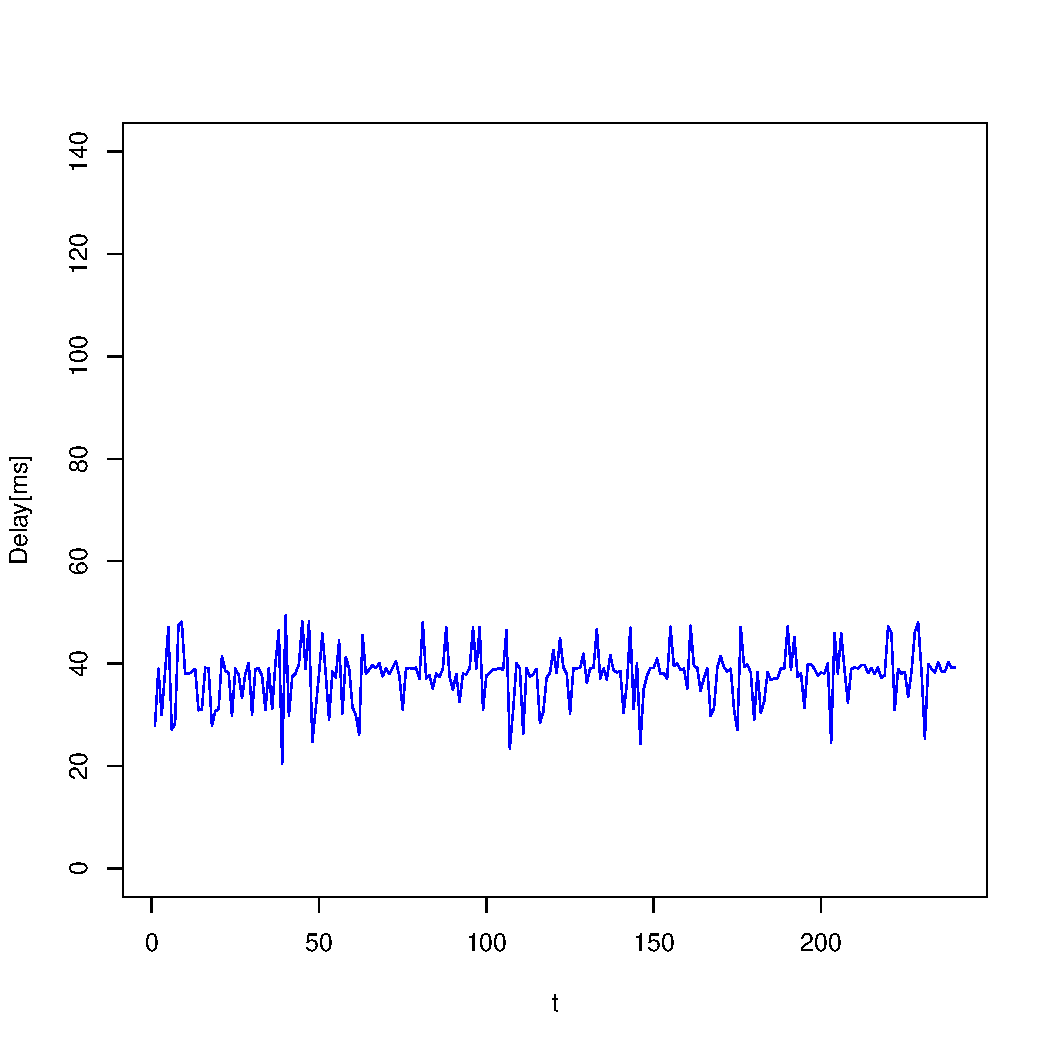
\includegraphics[width=.3\columnwidth]{C:/master/mstudy/analysis/plot/aws.amazon.com/20200226_070001-plot.pdf}
}~
\subfigure[12:00 - 13:00]{
\includegraphics[width=.3\columnwidth]{C:/master/mstudy/analysis/plot/aws.amazon.com/20200226_120001-plot.pdf}
}\\
\subfigure[17:00 - 18:00]{
\includegraphics[width=.3\columnwidth]{C:/master/mstudy/analysis/plot/aws.amazon.com/20200226_170001-plot.pdf}
}~
\subfigure[20:00 - 21:00]{
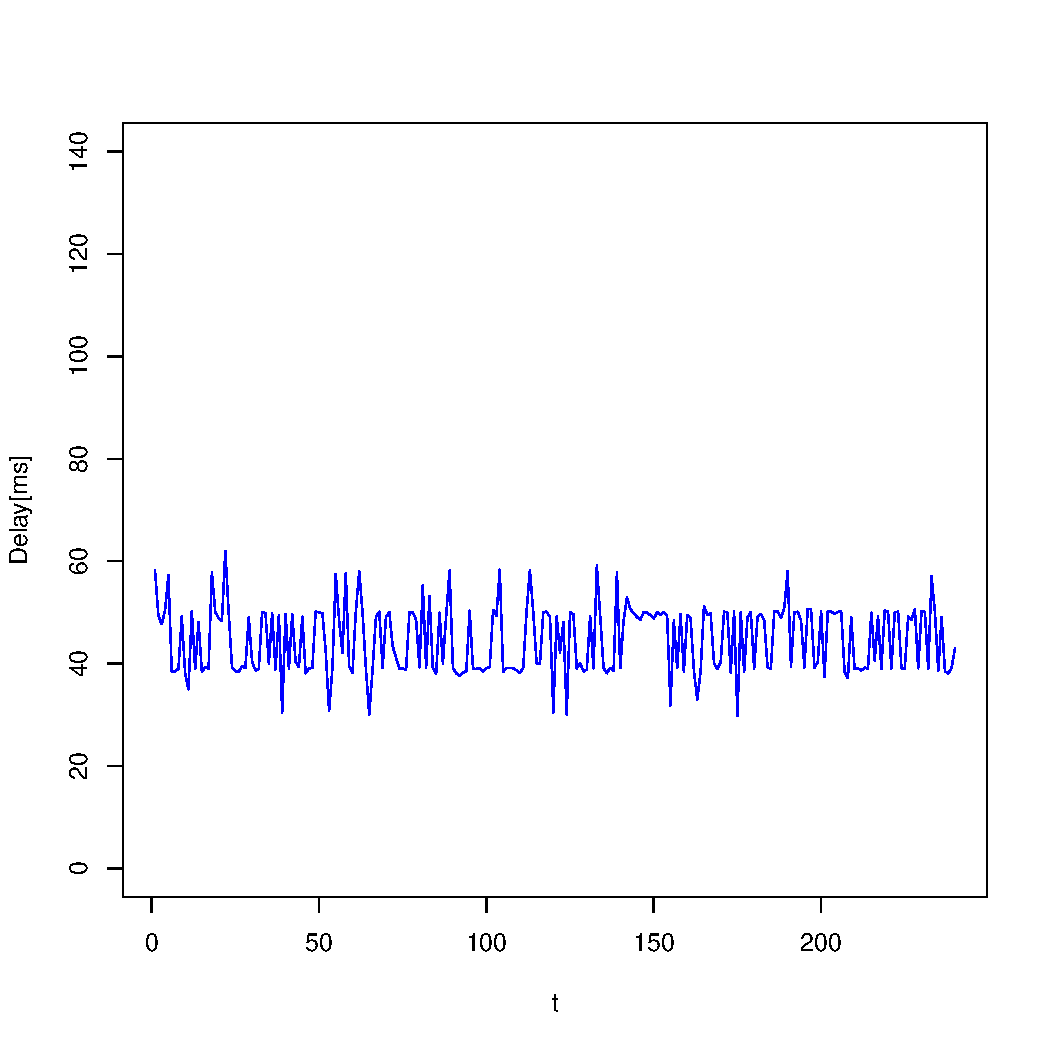
\includegraphics[width=.3\columnwidth]{C:/master/mstudy/analysis/plot/aws.amazon.com/20200226_200001-plot.pdf}
}
\caption{2月26日(水) aws.amazon.com を対象}

\subfigure[3:00 - 4:00]{
\includegraphics[width=.3\columnwidth]{C:/master/mstudy/analysis/plot/news.yahoo.co.jp/20200226_030001-plot.pdf}
}~
\subfigure[7:00 - 8:00]{
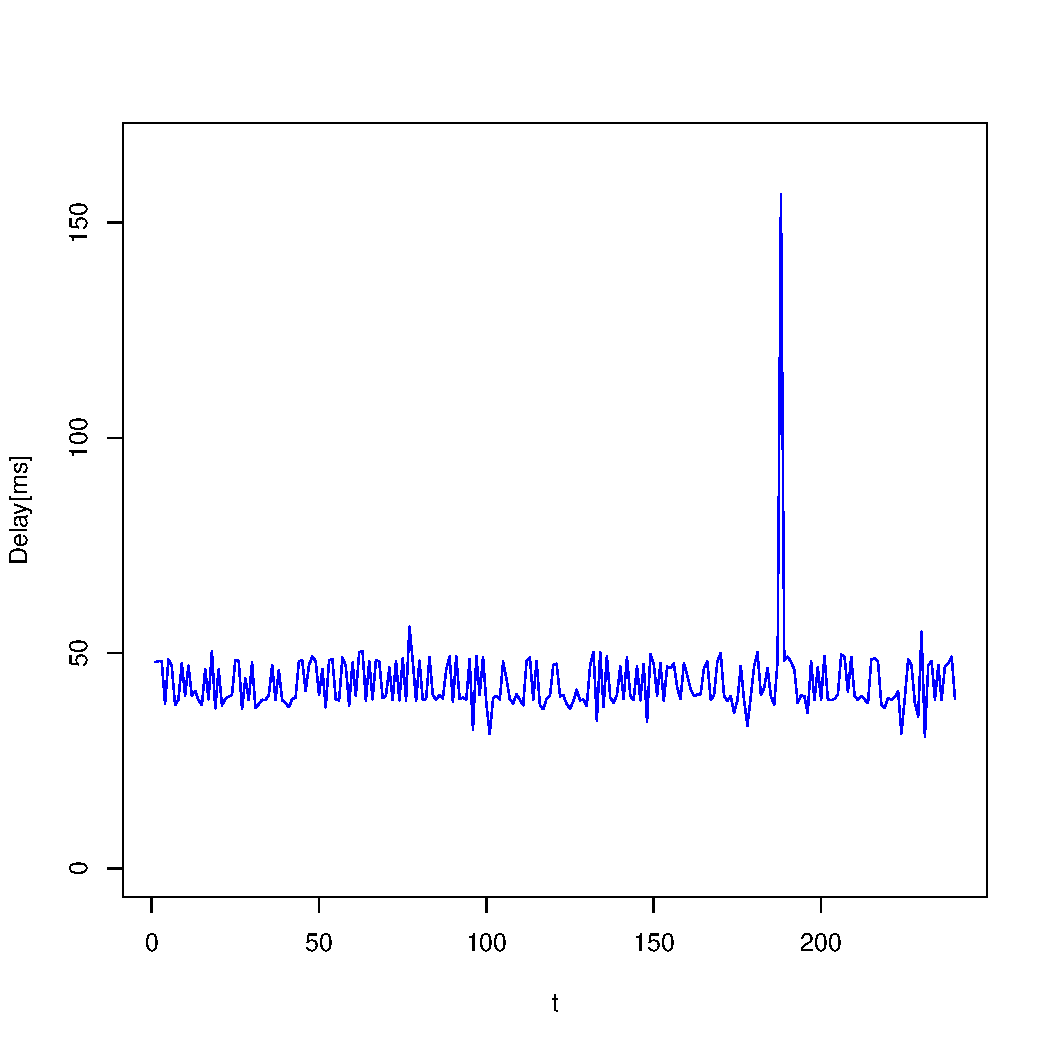
\includegraphics[width=.3\columnwidth]{C:/master/mstudy/analysis/plot/news.yahoo.co.jp/20200226_070002-plot.pdf}
}~
\subfigure[12:00 - 13:00]{
\includegraphics[width=.3\columnwidth]{C:/master/mstudy/analysis/plot/news.yahoo.co.jp/20200226_120001-plot.pdf}
}\\
\subfigure[17:00 - 18:00]{
\includegraphics[width=.3\columnwidth]{C:/master/mstudy/analysis/plot/news.yahoo.co.jp/20200226_170001-plot.pdf}
}~
\subfigure[20:00 - 21:00]{
\includegraphics[width=.3\columnwidth]{C:/master/mstudy/analysis/plot/news.yahoo.co.jp/20200226_200001-plot.pdf}
}
\caption{2月26日(水) news.yahoo.co.jp を対象}
\end{center}
\end{figure}

\begin{figure}[tb]
\begin{center}
\subfigure[3:00 - 4:00]{
\includegraphics[width=.3\columnwidth]{C:/master/mstudy/analysis/plot/aws.amazon.com/20200227_030001-plot.pdf}
}~
\subfigure[7:00 - 8:00]{
\includegraphics[width=.3\columnwidth]{C:/master/mstudy/analysis/plot/aws.amazon.com/20200227_070001-plot.pdf}
}~
\subfigure[12:00 - 13:00]{
\includegraphics[width=.3\columnwidth]{C:/master/mstudy/analysis/plot/aws.amazon.com/20200227_120001-plot.pdf}
}\\
\subfigure[17:00 - 18:00]{
\includegraphics[width=.3\columnwidth]{C:/master/mstudy/analysis/plot/aws.amazon.com/20200227_170001-plot.pdf}
}~
\subfigure[20:00 - 21:00]{
\includegraphics[width=.3\columnwidth]{C:/master/mstudy/analysis/plot/aws.amazon.com/20200227_200001-plot.pdf}
}
\caption{2月27日(木) aws.amazon.com を対象}

\subfigure[3:00 - 4:00]{
\includegraphics[width=.3\columnwidth]{C:/master/mstudy/analysis/plot/news.yahoo.co.jp/20200227_030001-plot.pdf}
}~
\subfigure[7:00 - 8:00]{
\includegraphics[width=.3\columnwidth]{C:/master/mstudy/analysis/plot/news.yahoo.co.jp/20200227_070001-plot.pdf}
}~
\subfigure[12:00 - 13:00]{
\includegraphics[width=.3\columnwidth]{C:/master/mstudy/analysis/plot/news.yahoo.co.jp/20200227_120001-plot.pdf}
}\\
\subfigure[17:00 - 18:00]{
\includegraphics[width=.3\columnwidth]{C:/master/mstudy/analysis/plot/news.yahoo.co.jp/20200227_170001-plot.pdf}
}~
\subfigure[20:00 - 21:00]{
\includegraphics[width=.3\columnwidth]{C:/master/mstudy/analysis/plot/news.yahoo.co.jp/20200227_200001-plot.pdf}
}
\caption{2月27日(木) news.yahoo.co.jp を対象}
\end{center}
\end{figure}

\begin{figure}[tb]
\begin{center}
\subfigure[3:00 - 4:00]{
\includegraphics[width=.3\columnwidth]{C:/master/mstudy/analysis/plot/aws.amazon.com/20200228_030002-plot.pdf}
}~
\subfigure[7:00 - 8:00]{
\includegraphics[width=.3\columnwidth]{C:/master/mstudy/analysis/plot/aws.amazon.com/20200228_070001-plot.pdf}
}~
\subfigure[12:00 - 13:00]{
\includegraphics[width=.3\columnwidth]{C:/master/mstudy/analysis/plot/aws.amazon.com/20200228_120001-plot.pdf}
}\\
\subfigure[17:00 - 18:00]{
\includegraphics[width=.3\columnwidth]{C:/master/mstudy/analysis/plot/aws.amazon.com/20200228_170002-plot.pdf}
}~
\subfigure[20:00 - 21:00]{
\includegraphics[width=.3\columnwidth]{C:/master/mstudy/analysis/plot/aws.amazon.com/20200228_200002-plot.pdf}
}
\caption{2月28日(金) aws.amazon.com を対象}

\subfigure[3:00 - 4:00]{
\includegraphics[width=.3\columnwidth]{C:/master/mstudy/analysis/plot/news.yahoo.co.jp/20200228_030001-plot.pdf}
}~
\subfigure[7:00 - 8:00]{
\includegraphics[width=.3\columnwidth]{C:/master/mstudy/analysis/plot/news.yahoo.co.jp/20200228_070002-plot.pdf}
}~
\subfigure[12:00 - 13:00]{
\includegraphics[width=.3\columnwidth]{C:/master/mstudy/analysis/plot/news.yahoo.co.jp/20200228_120001-plot.pdf}
}\\
\subfigure[17:00 - 18:00]{
\includegraphics[width=.3\columnwidth]{C:/master/mstudy/analysis/plot/news.yahoo.co.jp/20200228_170001-plot.pdf}
}~
\subfigure[20:00 - 21:00]{
\includegraphics[width=.3\columnwidth]{C:/master/mstudy/analysis/plot/news.yahoo.co.jp/20200228_200001-plot.pdf}
}
\caption{2月28日(金) news.yahoo.co.jp を対象}
\end{center}
\end{figure}

\begin{figure}[tb]
\begin{center}
\subfigure[3:00 - 4:00]{
\includegraphics[width=.3\columnwidth]{C:/master/mstudy/analysis/plot/AWS/20200229_030001-plot.pdf}
}~
\subfigure[7:00 - 8:00]{
\includegraphics[width=.3\columnwidth]{C:/master/mstudy/analysis/plot/AWS/20200229_070001-plot.pdf}
}~
\subfigure[12:00 - 13:00]{
\includegraphics[width=.3\columnwidth]{C:/master/mstudy/analysis/plot/AWS/20200229_120001-plot.pdf}
}\\
\subfigure[17:00 - 18:00]{
\includegraphics[width=.3\columnwidth]{C:/master/mstudy/analysis/plot/AWS/20200229_170002-plot.pdf}
}~
\subfigure[20:00 - 21:00]{
\includegraphics[width=.3\columnwidth]{C:/master/mstudy/analysis/plot/AWS/20200229_200001-plot.pdf}
}
\caption{2月29日(土) AWS サーバを対象}

\subfigure[3:00 - 4:00]{
\includegraphics[width=.3\columnwidth]{C:/master/mstudy/analysis/plot/news.yahoo.co.jp/20200229_030001-plot.pdf}
}~
\subfigure[7:00 - 8:00]{
\includegraphics[width=.3\columnwidth]{C:/master/mstudy/analysis/plot/news.yahoo.co.jp/20200229_070001-plot.pdf}
}~
\subfigure[12:00 - 13:00]{
\includegraphics[width=.3\columnwidth]{C:/master/mstudy/analysis/plot/news.yahoo.co.jp/20200229_120002-plot.pdf}
}\\
\subfigure[17:00 - 18:00]{
\includegraphics[width=.3\columnwidth]{C:/master/mstudy/analysis/plot/news.yahoo.co.jp/20200229_170001-plot.pdf}
}~
\subfigure[20:00 - 21:00]{
\includegraphics[width=.3\columnwidth]{C:/master/mstudy/analysis/plot/news.yahoo.co.jp/20200229_200001-plot.pdf}
}
\caption{2月29日(土) news.yahoo.co.jp を対象}
\end{center}
\end{figure}

\begin{figure}[tb]
\begin{center}
\subfigure[3:00 - 4:00]{
\includegraphics[width=.3\columnwidth]{C:/master/mstudy/analysis/plot/AWS/20200301_030001-plot.pdf}
}~
\subfigure[7:00 - 8:00]{
\includegraphics[width=.3\columnwidth]{C:/master/mstudy/analysis/plot/AWS/20200301_070002-plot.pdf}
}~
\subfigure[12:00 - 13:00]{
\includegraphics[width=.3\columnwidth]{C:/master/mstudy/analysis/plot/AWS/20200301_120001-plot.pdf}
}\\
\subfigure[17:00 - 18:00]{
\includegraphics[width=.3\columnwidth]{C:/master/mstudy/analysis/plot/AWS/20200301_170001-plot.pdf}
}~
\subfigure[20:00 - 21:00]{
\includegraphics[width=.3\columnwidth]{C:/master/mstudy/analysis/plot/AWS/20200301_200001-plot.pdf}
}
\caption{3月1日(日) AWS サーバを対象}

\subfigure[3:00 - 4:00]{
\includegraphics[width=.3\columnwidth]{C:/master/mstudy/analysis/plot/news.yahoo.co.jp/20200301_030001-plot.pdf}
}~
\subfigure[7:00 - 8:00]{
\includegraphics[width=.3\columnwidth]{C:/master/mstudy/analysis/plot/news.yahoo.co.jp/20200301_070001-plot.pdf}
}~
\subfigure[12:00 - 13:00]{
\includegraphics[width=.3\columnwidth]{C:/master/mstudy/analysis/plot/news.yahoo.co.jp/20200301_120001-plot.pdf}
}\\
\subfigure[17:00 - 18:00]{
\includegraphics[width=.3\columnwidth]{C:/master/mstudy/analysis/plot/news.yahoo.co.jp/20200301_170002-plot.pdf}
}~
\subfigure[20:00 - 21:00]{
\includegraphics[width=.3\columnwidth]{C:/master/mstudy/analysis/plot/news.yahoo.co.jp/20200301_200001-plot.pdf}
}
\caption{3月1日(日) news.yahoo.co.jp を対象}
\end{center}
\end{figure}

\begin{figure}[tb]
\begin{center}
\subfigure[3:00 - 4:00]{
\includegraphics[width=.3\columnwidth]{C:/master/mstudy/analysis/plot/AWS/20200302_030001-plot.pdf}
}~
\subfigure[7:00 - 8:00]{
\includegraphics[width=.3\columnwidth]{C:/master/mstudy/analysis/plot/AWS/20200302_070001-plot.pdf}
}~
\subfigure[12:00 - 13:00]{
\includegraphics[width=.3\columnwidth]{C:/master/mstudy/analysis/plot/AWS/20200302_120002-plot.pdf}
}\\
\subfigure[17:00 - 18:00]{
\includegraphics[width=.3\columnwidth]{C:/master/mstudy/analysis/plot/AWS/20200302_170001-plot.pdf}
}~
\subfigure[20:00 - 21:00]{
\includegraphics[width=.3\columnwidth]{C:/master/mstudy/analysis/plot/AWS/20200302_200001-plot.pdf}
}
\caption{3月2日(月) AWS サーバを対象}

\subfigure[3:00 - 4:00]{
\includegraphics[width=.3\columnwidth]{C:/master/mstudy/analysis/plot/news.yahoo.co.jp/20200302_030001-plot.pdf}
}~
\subfigure[7:00 - 8:00]{
\includegraphics[width=.3\columnwidth]{C:/master/mstudy/analysis/plot/news.yahoo.co.jp/20200302_070001-plot.pdf}
}~
\subfigure[12:00 - 13:00]{
\includegraphics[width=.3\columnwidth]{C:/master/mstudy/analysis/plot/news.yahoo.co.jp/20200302_120001-plot.pdf}
}\\
\subfigure[17:00 - 18:00]{
\includegraphics[width=.3\columnwidth]{C:/master/mstudy/analysis/plot/news.yahoo.co.jp/20200302_170001-plot.pdf}
}~
\subfigure[20:00 - 21:00]{
\includegraphics[width=.3\columnwidth]{C:/master/mstudy/analysis/plot/news.yahoo.co.jp/20200302_200001-plot.pdf}
}
\caption{3月2日(月) news.yahoo.co.jp を対象}
\end{center}
\end{figure}


\begin{figure}[tb]
\begin{center}
\subfigure[3:00 - 4:00]{
\includegraphics[width=.3\columnwidth]{C:/master/mstudy/analysis/plot/AWS/20200303_030001-plot.pdf}
}~
\subfigure[7:00 - 8:00]{
\includegraphics[width=.3\columnwidth]{C:/master/mstudy/analysis/plot/AWS/20200303_070001-plot.pdf}
}~
\subfigure[12:00 - 13:00]{
\includegraphics[width=.3\columnwidth]{C:/master/mstudy/analysis/plot/AWS/20200303_120001-plot.pdf}
}\\
\subfigure[17:00 - 18:00]{
\includegraphics[width=.3\columnwidth]{C:/master/mstudy/analysis/plot/AWS/20200303_170001-plot.pdf}
}~
\subfigure[20:00 - 21:00]{
\includegraphics[width=.3\columnwidth]{C:/master/mstudy/analysis/plot/AWS/20200303_200001-plot.pdf}
}
\caption{3月3日(火) AWS サーバを対象}

\subfigure[3:00 - 4:00]{
\includegraphics[width=.3\columnwidth]{C:/master/mstudy/analysis/plot/news.yahoo.co.jp/20200303_030001-plot.pdf}
}~
\subfigure[7:00 - 8:00]{
\includegraphics[width=.3\columnwidth]{C:/master/mstudy/analysis/plot/news.yahoo.co.jp/20200303_070001-plot.pdf}
}~
\subfigure[12:00 - 13:00]{
\includegraphics[width=.3\columnwidth]{C:/master/mstudy/analysis/plot/news.yahoo.co.jp/20200303_120001-plot.pdf}
}\\
\subfigure[17:00 - 18:00]{
\includegraphics[width=.3\columnwidth]{C:/master/mstudy/analysis/plot/news.yahoo.co.jp/20200303_170001-plot.pdf}
}~
\subfigure[20:00 - 21:00]{
\includegraphics[width=.3\columnwidth]{C:/master/mstudy/analysis/plot/news.yahoo.co.jp/20200303_200002-plot.pdf}
}
\caption{3月3日(火) news.yahoo.co.jp を対象}
\label{data-end}
\end{center}
\end{figure}

aws.amazon.com を対象とした計測データの平均値は 38ms から 42ms 程度であった.
また,特徴的な計測データとして,図 \ref{aws} のように比較的遅延変動が起こりにくいものが見て取れた.
traceroute の結果は,2/22(土)3:00 から 2/23(日)13:00 までと,2/25(火)17:00 から 2/28(金)21:00 までは主に
\begin{table}[H]
\centering
\begin{tabular}{l}
 1  *\\
 2  *\\
 3  osk004ix51.IIJ.Net (58.138.106.126)\\
 4  210.173.178.59 (210.173.178.59) , 210.173.178.61 (210.173.178.61)\\
 5  *\\
 6  *\\
 7  *\\
 8  *\\
 9  *\\
10  *\\
11  *\\
12  server-13-224-139-70.nrt51.r.cloudfront.net (13.224.139.70)\\
\end{tabular}
\end{table}
となっていた.
4 ホップ目はともに大阪にある IX である.
2/23(日)17:00 から 2/25(火)13:00までは主に
\begin{table}[H]
\centering
\begin{tabular}{l}
 1  *\\
 2  tky008nasgw110.IIJ.Net (160.13.52.245)\\
 3  *\\
 4  tky001bb10.IIJ.Net (58.138.88.1)\\
 5  tky001ix15.IIJ.Net (58.138.102.210)\\
 6  210.173.176.188 (210.173.176.188) , 210.173.176.198 (210.173.176.198)\\
 7  *\\
 8  52.95.30.16 (52.95.30.16) , 52.95.30.18 (52.95.30.18) , ...\\
 9  *\\
10  *\\
11  *\\
12  *\\
13  *\\
14  *\\
15  *\\
16  server-54-230-172-71.nrt57.r.cloudfront.net (54.230.172.71)\\
\end{tabular}
\end{table}
となっていた.
6 ホップ目はともに東京にある IX であり,8 ホップ目は全て東京にある Amazon のネットワーク内の機器であり所在地は日本であった.

news.yahoo.co.jp を対象とした計測データの平均値は,42ms から 45ms 程度であった.
traceroute による経路だが,
\begin{table}[H]
\centering
\begin{tabular}{l}
 1  *\\
 2  tky008nasgw110.IIJ.Net (160.13.52.241)\\
 3  *\\
 4  *\\
 5  osk004ip56.IIJ.Net (58.138.106.154)\\
 6  210.138.106.238 (210.138.106.238)\\
 7  183.79.224.146 (183.79.224.146)\\
 8  183.79.250.123 (183.79.250.123)\\
や\\
 1  *\\
 2  tky008nasgw110.IIJ.Net (160.13.52.245)\\
 3  *\\
 4  tky001bb10.IIJ.Net (58.138.88.1)\\
 5  tky001ix50.IIJ.Net (58.138.102.34)\\
 6  210.130.154.162 (210.130.154.162)\\
 7  *\\
 8  182.22.25.124 (182.22.25.124)\\
\end{tabular}
\end{table}
などが入り混じっていた.
yahoo ニュースのウェブサーバは負荷分散を行っているようで ping や traceroute の宛先をドメイン名で指定してしまったため,計測毎に異なるサーバに対しコマンド実行を行ってしまった.
今後は IP アドレス指定で計測を行います.
 
AWS サーバを対象とした計測データの平均値は,70ms 前半のものと 80ms 後半のものが見て取れる.
また,特徴として単発的に 40ms 程度の小さな応答遅延が発生するようだ.
traceroute による経路は,2/29(土)3:00 から 2/29(土)13:00 までは
\begin{table}[H]
\centering
\begin{tabular}{l}
 1  *\\
 2  *\\
 3  osk004ix50.IIJ.Net (58.138.106.122)\\
 4  210.173.178.59 (210.173.178.59)\\
 5  *\\
 6  *\\
 7  *\\
 8  54.239.53.47 (54.239.53.47)\\
 9  *\\
10  *\\
11  52.95.31.219 (52.95.31.219)\\
12  *\\
13  *\\
14  52.95.30.220 (52.95.30.220)\\
15  *\\
16  *\\
============\\
120 *\\
\end{tabular}
\end{table}
となっており,2/29(土)17:00 から 3/3(火)21:00 までは
\begin{table}[H]
\centering
\begin{tabular}{l}
 1  *\\
 2  tky008nasgw110.IIJ.Net (160.13.52.241)\\
 3  *\\
 4  tky001bb10.IIJ.Net (58.138.88.1)\\
 5  tky001ix11.IIJ.Net (58.138.101.2)\\
 6  210.173.176.188 (210.173.176.188)\\
 7  *\\
 8  *\\
 9  *\\
10  *\\
11  *\\
12  *\\
13  *\\
14  *\\
15  52.95.31.197 (52.95.31.197)\\
16  *\\
17  *\\
18  52.95.30.208 (52.95.30.208)\\
19  *\\
=============\\
120  *\\
\end{tabular}
\end{table}
となっていた.
IP アドレス 52.95.30.0 から 52.95.31.255 は Amazon のネットワーク内の機器であり所在地は日本である.
また,原因はよくわからないのですが,120 ホップまででは AWS サーバから traceroute の応答が得られませんでした.
\section{fBmモデル}
fBm モデルは長期依存性を持つ時系列モデルとして知られており,通信トラフィックのモデル化などに使用された\cite{rizk2012non}.
これは測定データを $\{y_t\}$ として次式で表される\cite{perrin2002fast}.
$$y_t = B(t) - B(t-1)$$
$$B(t) \sim N(0,\sigma^2)$$
$$\textbf{E}[B(t)-B(s)] = 0$$
$$\textbf{E}[(B(t)-B(s))^2] = \sigma^2|t-s|^{2H}$$
$$0<H<1$$
このパラメータは$ H と \sigma^2 $だと思います.まだ理解しきれていないので,これからパラメータ推定を行います. 
\section{今後の予定}
\begin{itemize}
\item ポスターを作成します.
\item 卒論の内容をもとに IN の原稿を執筆します.改善点として,パラメータの次数決めにおいて AIC の代わりに WBIC\cite{watanabe2013waic} などの他の情報量基準を用いることや,モデルの適合度の評価において,リュング・ボックス検定\cite{asai1999ana}などの検定を行うことを考えています.ただ今回の計測データは SINET のウェブサーバを対象とした計測データと同様,生データで曜日や時間帯ごとに応じた顕著な傾向が見れているわけではないので,卒論と同じ時系列データを用いた傾向分析がうまくいくのか怪しいと思っています.分布に注目した確率モデル,確率遷移モデルといった別のアプローチも試してみたほうが良いのかとも思っているのですが,ご意見をいただきたいです.
\end{itemize}
\section{スケジュール}
\begin{table}[H]
\begin{tabular}{|c|c|}
\hline
日付&予定\\
\hline
3/21&ポスター完成\\
\hline
3/31&ポスター締め切り\\
\hline
4/1&原稿書き上げ\\
\hline
4月中旬&原稿締め切り\\
\hline
5/21 - 5/22&IN研究会\\
\hline
\end{tabular}
\end{table}
原稿執筆後 : 抄録とキーワードの登録(日本語と英語)

プログラム決定後 : 参加費支払い

5/14~ : 技報ダウンロード開始

\bibliography{reference}
\bibliographystyle{ieeetr}
\end{document}